\section{Date: 2026-09-07}
\noindent \textbf{Series ID: WPDILTU} 

\noindent This series is titled Discussion About Pandemics Index for Lithuania and has a frequency of Quarterly. The units are Index and the seasonal adjustment is Not Seasonally Adjusted.The observation start date is 1996-01-01 and the observation end date is 2026-04-01.The popularity of this series is 1. \\ 

\noindent \textbf{Series ID: MTSMFBP133FMS} 

\noindent This series is titled Means of Financing: Borrowing from the Public and has a frequency of Monthly. The units are Millions of Dollars and the seasonal adjustment is Not Seasonally Adjusted.The observation start date is 2010-01-01 and the observation end date is 2026-07-01.The popularity of this series is 14. \\ 

\subsection{Raw Regression}
\noindent Regresses the two series against each other directly. A significant result here can come just as easily from both series sharing a long-run trend as from any real relationship.

\begin{center}
\begin{tabular}{lclc}
\toprule
\textbf{Dep. Variable:}       & value\_fred\_MTSMFBP133FMS & \textbf{  R-squared:         } &     0.199   \\
\textbf{Model:}               &            OLS             & \textbf{  Adj. R-squared:    } &     0.186   \\
\textbf{Method:}              &       Least Squares        & \textbf{  F-statistic:       } &     15.87   \\
\textbf{Date:}                &      Mon, 07 Sep 2026      & \textbf{  Prob (F-statistic):} &  0.000176   \\
\textbf{Time:}                &          16:43:46          & \textbf{  Log-Likelihood:    } &   -893.46   \\
\textbf{No. Observations:}    &               66           & \textbf{  AIC:               } &     1791.   \\
\textbf{Df Residuals:}        &               64           & \textbf{  BIC:               } &     1795.   \\
\textbf{Df Model:}            &                1           & \textbf{                     } &             \\
\textbf{Covariance Type:}     &         nonrobust          & \textbf{                     } &             \\
\bottomrule
\end{tabular}
\begin{tabular}{lcccccc}
                              & \textbf{coef} & \textbf{std err} & \textbf{t} & \textbf{P$> |$t$|$} & \textbf{[0.025} & \textbf{0.975]}  \\
\midrule
\textbf{const}                &    4.886e+04  &     2.46e+04     &     1.985  &         0.051        &     -321.644    &      9.8e+04     \\
\textbf{value\_fred\_WPDILTU} &    1205.6312  &      302.613     &     3.984  &         0.000        &      601.092    &     1810.170     \\
\bottomrule
\end{tabular}
\begin{tabular}{lclc}
\textbf{Omnibus:}       & 51.230 & \textbf{  Durbin-Watson:     } &    2.093  \\
\textbf{Prob(Omnibus):} &  0.000 & \textbf{  Jarque-Bera (JB):  } &  275.412  \\
\textbf{Skew:}          &  2.139 & \textbf{  Prob(JB):          } & 1.57e-60  \\
\textbf{Kurtosis:}      & 12.047 & \textbf{  Cond. No.          } &     87.5  \\
\bottomrule
\end{tabular}
%\caption{OLS Regression Results}
\end{center}

Notes: \newline
 [1] Standard Errors assume that the covariance matrix of the errors is correctly specified.

\begin{figure}
\centering
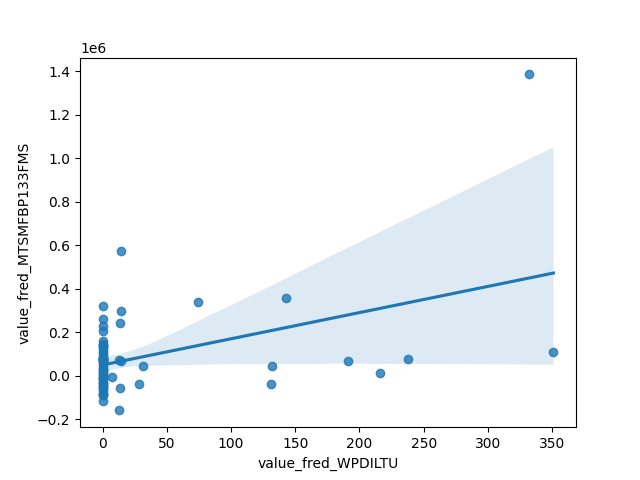
\includegraphics[scale = 0.9]{plots/plot_2026-09-07.png}
\caption{Raw Regression Plot for 2026-09-07}
\end{figure}
\newpage
\subsection{Detrended Regression}
\noindent Regresses the residuals of each series after removing its own linear time trend, so a shared trend can no longer drive the result on its own. A relationship that stays significant here is better evidence of a genuine link between the two series.

\begin{center}
\begin{tabular}{lclc}
\toprule
\textbf{Dep. Variable:}                  & value\_fred\_MTSMFBP133FMS\_detrended & \textbf{  R-squared:         } &     0.174   \\
\textbf{Model:}                          &                  OLS                  & \textbf{  Adj. R-squared:    } &     0.161   \\
\textbf{Method:}                         &             Least Squares             & \textbf{  F-statistic:       } &     13.48   \\
\textbf{Date:}                           &            Mon, 07 Sep 2026           & \textbf{  Prob (F-statistic):} &  0.000493   \\
\textbf{Time:}                           &                16:43:46               & \textbf{  Log-Likelihood:    } &   -893.06   \\
\textbf{No. Observations:}               &                     66                & \textbf{  AIC:               } &     1790.   \\
\textbf{Df Residuals:}                   &                     64                & \textbf{  BIC:               } &     1794.   \\
\textbf{Df Model:}                       &                      1                & \textbf{                     } &             \\
\textbf{Covariance Type:}                &               nonrobust               & \textbf{                     } &             \\
\bottomrule
\end{tabular}
\begin{tabular}{lcccccc}
                                         & \textbf{coef} & \textbf{std err} & \textbf{t} & \textbf{P$> |$t$|$} & \textbf{[0.025} & \textbf{0.975]}  \\
\midrule
\textbf{const}                           &    5.051e-09  &     2.28e+04     &  2.22e-13  &         1.000        &    -4.55e+04    &     4.55e+04     \\
\textbf{value\_fred\_WPDILTU\_detrended} &    1138.7087  &      310.105     &     3.672  &         0.000        &      519.204    &     1758.214     \\
\bottomrule
\end{tabular}
\begin{tabular}{lclc}
\textbf{Omnibus:}       & 52.012 & \textbf{  Durbin-Watson:     } &    2.129  \\
\textbf{Prob(Omnibus):} &  0.000 & \textbf{  Jarque-Bera (JB):  } &  302.597  \\
\textbf{Skew:}          &  2.138 & \textbf{  Prob(JB):          } & 1.96e-66  \\
\textbf{Kurtosis:}      & 12.579 & \textbf{  Cond. No.          } &     73.4  \\
\bottomrule
\end{tabular}
%\caption{OLS Regression Results}
\end{center}

Notes: \newline
 [1] Standard Errors assume that the covariance matrix of the errors is correctly specified.

\begin{figure}
\centering
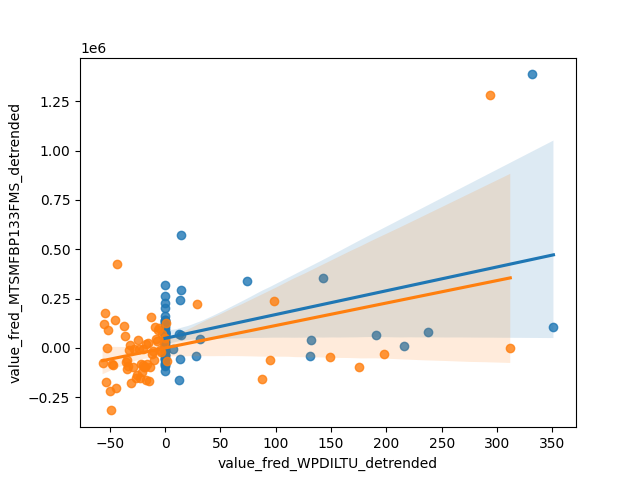
\includegraphics[scale = 0.9]{plots/plot_2026-09-07_detrended.png}
\caption{Detrended Regression Plot for 2026-09-07}
\end{figure}
\newpage
